\documentclass[12pt]{article}
\usepackage{amsmath}
\usepackage{listings}
\usepackage{color}
\usepackage{graphicx}
\usepackage{bm}
\usepackage[margin=0.5in]{geometry}

\title{Homework 1}
\author{Dan Kolbman}
\date{October 20, 2014}

\definecolor{mygreen}{rgb}{0,0.6,0}
\definecolor{mygray}{rgb}{0.95,0.95,0.95}
\definecolor{mymauve}{rgb}{0.58,0,0.82}
%\definecolor{mygray}{RGB}{22, 22, 22}}

\lstset{ %
  language=Python,
  backgroundcolor=\color{mygray},   % choose the background color
  basicstyle=\footnotesize,        % size of fonts used for the code
  breaklines=true,                 % automatic line breaking only at whitespace
  captionpos=b,                    % sets the caption-position to bottom
  commentstyle=\color{mygreen},    % comment style
  %escapeinside={\%*}{*)},          % if you want to add LaTeX within your code
  keywordstyle=\color{blue},       % keyword style
  stringstyle=\color{mymauve},     % string literal style
  frame=L,
  xleftmargin=\parindent,
  showstringspaces=false
}
\begin{document}
  
  \maketitle
  %\lstinputlisting{Problem1.out}

  %\begin{figure}[h!]
  %  \centering
  %  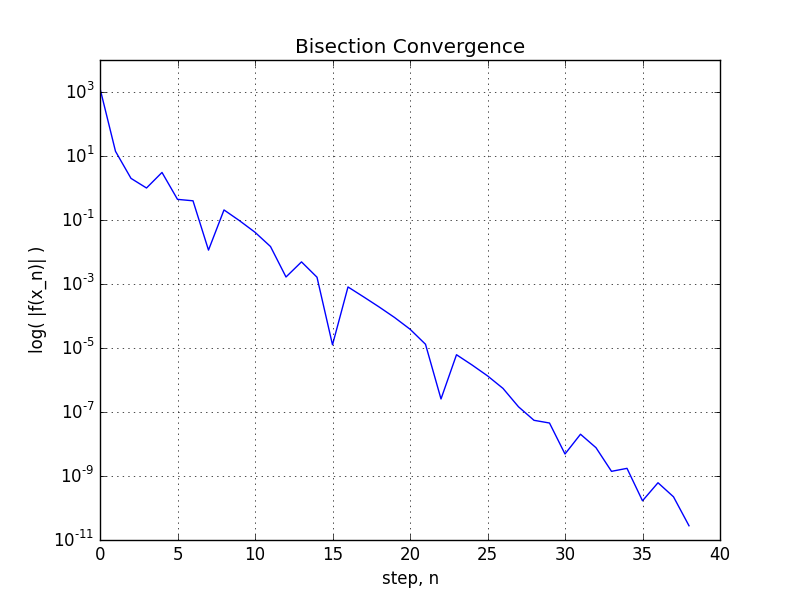
\includegraphics[width=0.5\textwidth]{Problem4a.png}
  %  \caption{(Approximately) Quadratic Convergence}
  %\end{figure}
 
  \section{Finite Differencing in Curved Coordinates}

  \section{Differentiation and Integration with Noise}


  \begin{align}
    f(x) &= sin(x)e^{cos(x)} \\
    f^{\prime}(x) &= (cos(x)-sin^2(x))e^{cos(x)}
  \end{align}

  \subsection{Differentiation using Stencils}
  \begin{figure}[h!]
    \centering
    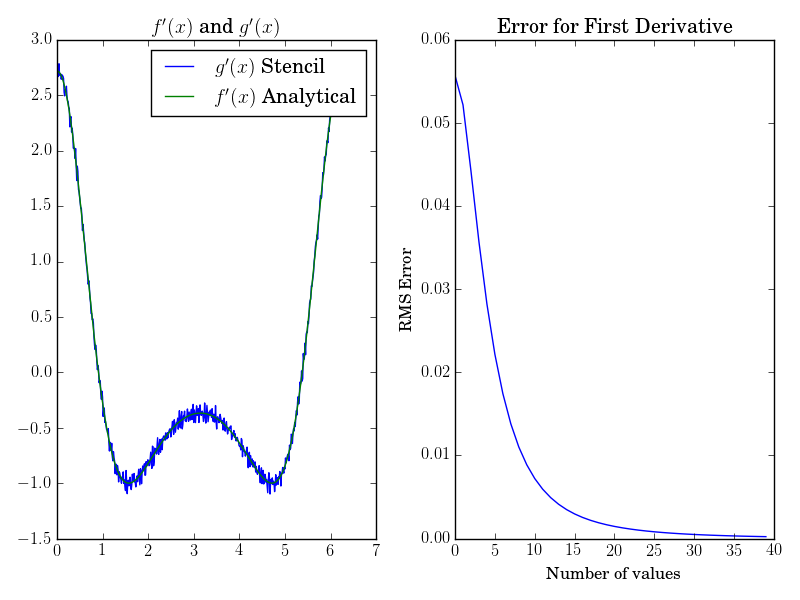
\includegraphics[width=0.8\textwidth]{Problem2ia.png}
    \caption{RMS Error in 5 point stencil for the first derivative}
  \end{figure}

  \begin{figure}[h!]
    \centering
    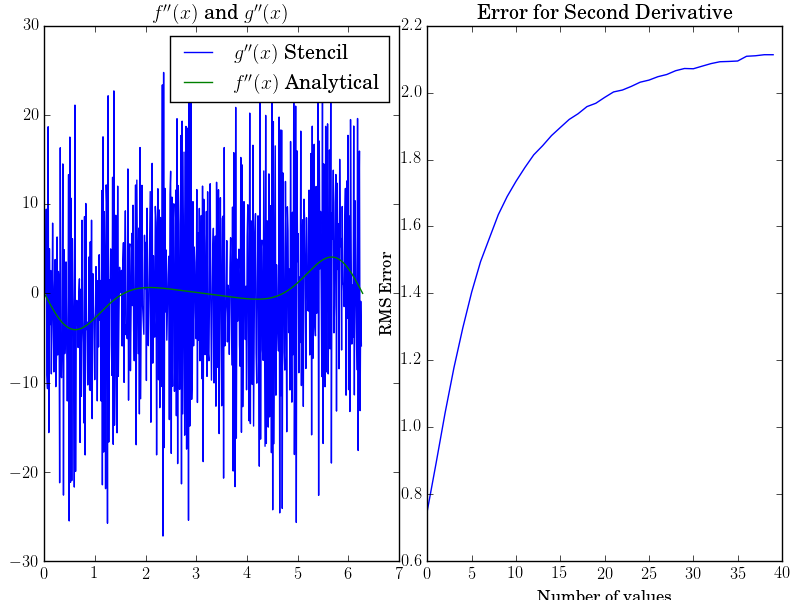
\includegraphics[width=0.8\textwidth]{Problem2ib.png}
    \caption{RMS Error in 5 point stencil for the second derivative}
  \end{figure}

  \subsection{Integration with Simpson's Rule}
  
  \begin{figure}[h!]
    \centering
    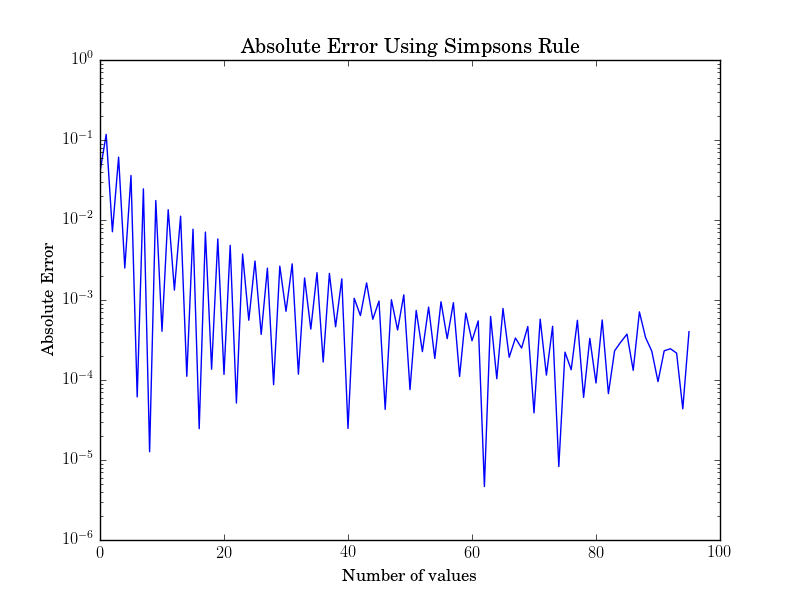
\includegraphics[width=0.8\textwidth]{Problem2ii.png}
    \caption{RMS Error using Simpson's Rule for varying numbers of points}
  \end{figure}

  \section{Cepheid Lightcurve Integraiton}

  \section{Planck's Law}

  \section{Romberg Integration}

\end{document}
